\pdfoutput=1
\pdfcompresslevel=9
\pdfinfo
{
    /Author (Michał Herman)
    /Title (RSO Projekt)
    /Subject (RSO Projekt)
    /Keywords (RSO)
}
%\documentclass[a4paper,polish,onecolumn,twoside,floatssmall,11pt,titleauthor,wide,openright]{mwrep}
%\usepackage[scale={0.7,0.8},paper=a4paper,twoside]{geometry}
\documentclass[a4paper,onecolumn,oneside,11pt,wide,floatssmall]{mwrep}
% \usepackage{polish}
\usepackage{amsmath}
\usepackage{amsfonts}
\usepackage{amssymb}
\usepackage{amsthm}
\usepackage{bookman}
\usepackage{tabto}
\usepackage{longtable}
\usepackage{enumitem}
\usepackage{tabularx}
\usepackage{multirow}

\usepackage{geometry}
\usepackage[utf8x]{inputenc}
\usepackage[T1]{fontenc}
% \usepackage{t1enc}
% \usepackage[pdftex, bookmarks]{hyperref}
\usepackage[pdftex, bookmarks=false]{hyperref}
\usepackage[titletoc,title]{appendix}
\def\url#1{{ \tt #1}}

\usepackage{listings}

% marginesy
\textwidth\paperwidth
\advance\textwidth -55mm
\oddsidemargin-0.9in
\advance\oddsidemargin 33mm
\evensidemargin-0.9in
\advance\evensidemargin 33mm
\topmargin -1in
\advance\topmargin 25mm
\setlength\textheight{48\baselineskip}
\addtolength\textheight{\topskip}
\marginparwidth15mm

\clubpenalty=10000 % to kara za sierotki
\widowpenalty=10000 % nie pozostawia wdów
\brokenpenalty=10000 % nie dzieli wyrazów pomiędzy stronami
\sloppy

\tolerance4500
\pretolerance250
\hfuzz=1.5pt
\hbadness1450

% ŻYWA PAGINA
\renewcommand{\chaptermark}[1]{\markboth{\scshape\small\bfseries \
#1}{\small\bfseries \ #1}}
\renewcommand{\sectionmark}[1]{\markboth{\scshape\small\bfseries\thesection.\
#1}{\small\bfseries\thesection.\ #1}}
\newcommand{\headrulewidth}{0.5pt}
\newcommand{\footrulewidth}{0.pt}
\pagestyle{uheadings}

\usepackage[pdftex]{color,graphicx}
\usepackage[polish]{babel}

% \textheight232mm
% \setlength{\textwidth}{\textwidth}
% \setlength{\oddsidemargin}{\evensidemargin}
% \setlength{\evensidemargin}{0.3cm}
\usepackage[sort, compress]{cite}
\usepackage{pdfpages}

%\usepackage{multibib}
%\newcites{bk,st,doc,web}{Książki i~artykuły,Standardy i~zalecenia,Dokumentacja produktów,Publikacje i~serwisy internetowe}

\theoremstyle{definition}
\newtheorem{defn}{Definicja}[section]
\newtheorem{conj}{Teza}[section]
\newtheorem{conjmain}{Teza}
\newtheorem{exmp}{Przykład}[section]

\theoremstyle{plain}% default
\newtheorem{thm}{Twierdzenie}[section]
\newtheorem{lem}[thm]{Lemat}
\newtheorem{prop}[thm]{Hipoteza}
\newtheorem*{cor}{Wniosek}

\theoremstyle{remark}
\newtheorem*{rem}{Uwaga}
\newtheorem*{note}{Uwaga}
\newtheorem{case}{Przypadek}

\definecolor{ListingBackground}{rgb}{0.95,0.95,0.95}
%\renewcommand{\familydefault}{\sfdefault} % font
\begin{document}

% kody źródłowe wplatane w tekst
\lstdefinestyle{incode}
{
basicstyle={\footnotesize},
keywordstyle={\bf\footnotesize\color{black}},
commentstyle={\em\footnotesize\color{magenta}},
numbers=left,
stepnumber=5,
firstnumber=1,
numberfirstline=true,
numberblanklines=true,
numberstyle={\sf\tiny},
numbersep=10pt,
tabsize=2,
xleftmargin=17pt,
framexleftmargin=3pt,
framexbottommargin=2pt,
framextopmargin=2pt,
framexrightmargin=0pt,
showstringspaces=true,
backgroundcolor={\color{ListingBackground}},
extendedchars=true,
% title=\lstname,
captionpos=b,
% abovecaptionskip=1pt,
% belowcaptionskip=1pt,
frame=tb,
framerule=0pt,
}

% kody źródłowe z podpisem
\lstdefinestyle{outcode}
{
basicstyle={\footnotesize},
keywordstyle={\bf\footnotesize\color{black}},
commentstyle={\em\footnotesize\color{magenta}},
numbers=left,
stepnumber=5,
firstnumber=1,
numberfirstline=true,
numberblanklines=true,
numberstyle={\sf\tiny},
numbersep=10pt,
tabsize=2,
xleftmargin=17pt,
framexleftmargin=3pt,
framexbottommargin=2pt,
framextopmargin=2pt,
framexrightmargin=0pt,
showstringspaces=true,
backgroundcolor={\color{ListingBackground}},
extendedchars=true,
% title=\lstname,
captionpos=b,
% abovecaptionskip=1pt,
% belowcaptionskip=1pt,
frame=tb,
framerule=0.1pt,
}

\renewcommand*\lstlistingname{Wydruk}
\renewcommand*\lstlistlistingname{Spis wydruków}
\renewcommand{\labelitemii}{$\bullet$}

\pagenumbering{roman}
\renewcommand{\baselinestretch}{1.0}
\raggedbottom

\begin{titlepage}
    % Strona tytułowa
    \vbox to\textheight{\hyphenpenalty=10000
    \begin{center}
	\begin{tabular}{p{107mm} p{9cm}}
	    \begin{minipage}{9cm}
	      \begin{center}
	      Politechnika Warszawska \\
	      Wydział Elektroniki i~Technik Informacyjnych
	      \end{center}
	    \end{minipage}
	    &
	    \begin{minipage}{8cm}
	    \begin{flushleft}
	     \footnotesize
	      Rok akademicki 2016/2017
	    \vspace*{2.75\baselineskip}
	    \end{flushleft}
	    \end{minipage} \\
	\end{tabular}
	\vspace*{3.75\baselineskip}
	\par\vspace{\smallskipamount}
	%\vspace*{2\baselineskip}{\LARGE Projekt RSO\par}
	\vspace{3\baselineskip}{\LARGE\strut 
	Tomasz Rydzewski \\
	Magdalena Malenda \\
	Joanna Ohradka \\
	Włodzimierz Szewczyk \\
	Piotr Kuciński \\
	Dominik Giżyński \\
	Michał Herman
	\par}
	\vspace*{2\baselineskip}{\huge\bfseries Projekt RSO\par}

	\vspace*{7\baselineskip}
	\hfill\mbox{}\par\vspace*{\baselineskip}\noindent
	\begin{tabular}[b]{@{}p{3cm}@{\ }l@{}}
	    {\large\hfill } & {\large }
	\end{tabular}
	\hfil
    \end{center}}


\end{titlepage}

% ex: set tabstop=4 shiftwidth=4 softtabstop=4 noexpandtab fileformat=unix filetype=tex spelllang=pl,en spell:


\tableofcontents
% \addcontentsline{toc}{chapter}{{Przedmowa1}{vii}}{vii}

% \chapter*{Spis tablic, rysunków i~wydruków}
% \listoftables
% \listoffigures
% \lstlistoflistings

%\setlength{\baselineskip}{7mm}
\newpage
\pagenumbering{arabic}
\setcounter{page}{1}

\chapter{Projekt}


\section{Harmonogram}
Poniżej przedstawiony został harmonogram projektu wraz z diagramem Gantta.

  \begin{longtable}{| p{.40\textwidth} || p{.25\textwidth} | p{.25\textwidth} |}
\hline
\textbf{Nazwa zadania} & \textbf{Data rozpoczęcia} & \textbf{Data zakończenia} \\ \hline
Organizacja struktury projektu & 16-03-21 & 16-03-29 \\ \hline
Pierwsze spotkanie projektowe & 16-03-31 & 16-03-31 \\ \hline
Wystartowanie repozytorium Git & 16-04-01 & 16-04-04 \\ \hline
Ustalenia funkcjonalne i niefunkcjonalne & 16-04-01 & 16-04-05 \\ \hline
Utworzenie koncepcji architektury systemu & 16-04-01 & 16-04-20 \\ \hline
Utworzenie koncepcji wykorzystania narzędzia docker & 16-04-01 & 16-04-20 \\ \hline
Utworzenie dokumentu dobrych praktyk & 16-04-15 & 16-04-21 \\ \hline
Utworzenie tutoriala docker & 16-04-18 & 16-04-21 \\ \hline
Dodanie rozwiązania docker do repozytorium & 16-04-19 & 16-04-20 \\ \hline
Doprecyzowanie wymagań przedmiotu & 16-04-19 & 16-04-20 \\ \hline
Wybranie algorytmów & 16-04-19 & 16-04-20 \\ \hline
Ustalenie prezentacji na drugi krok milowy & 16-04-21 & 16-04-21 \\ \hline
Modułowy podział projektu & 16-04-21 & 16-04-22 \\ \hline
Szczegłowa koncepcja rozwiązania & 16-04-25 & 16-04-28 \\ \hline
Ustawienie środowiska programistycznego & 16-04-20 & 16-04-20 \\ \hline
Utworzenie pierwszych scenariuszy testowych (do prezentacji pierwszego kroku milowego) & 16-04-19 & 16-04-22 \\ \hline
Ustalenie wykorzystywanej bazy danych & 16-04-21 & 16-04-25 \\ \hline
Postawienie bazy danych & 16-04-26 & 16-04-27 \\ \hline
Część programistyczna & 16-04-25 & 16-06-03 \\ \hline
Zebranie dokumentacji na pierwszy krok & 16-04-22 & 16-04-22 \\ \hline
I krok milowy & 16-04-29 & 16-04-29 \\ \hline
Utworzenie wszystkich scenariuszy testowych & 16-04-25 & 16-05-03 \\ \hline
Odłożenie bruncha na II krok milowy & 16-04-29 & 16-04-29 \\ \hline
II krok milowy & 16-05-06 & 16-05-06 \\ \hline
Ustalenie prezentacji na trzeci krok milowy & 16-05-09 & 16-05-11 \\ \hline
Testy bezpieczeństwa & 16-05-30 & 16-06-03 \\ \hline
Testy fukcjonalne & 16-05-30 & 16-06-03 \\ \hline
Testy awaryjności & 16-05-30 & 16-06-03 \\ \hline
III krok milowy & 16-06-10 & 16-06-10 \\ \hline
Doprecyzowanie wymagań funkcjonalnych systemu & 16-05-05 & 16-05-06 \\ \hline
Doprecyzowanie wymagań niefunkcjonalnych systemu & 16-05-10 & 16-05-13 \\ \hline
Doprecyzowanie architektury systemu & 16-05-10 & 16-05-16 \\ \hline
Opracowanie pełnego planu testów & 16-05-09 & 16-05-20 \\ \hline
Opracowanie scenariusza końcowej prezentacji & 16-05-09 & 16-05-20 \\ \hline
Wyodrębnienie głównych elementów systemu & 16-05-15 & 16-05-15 \\ \hline
Określenie sposobu lokalnego developmentu aplikacji & 16-05-15 & 16-05-16 \\ \hline
Klient - użytkownik & 16-05-15 & 16-05-16 \\ \hline
Klient do wprowadzania danych & 16-05-20 & 16-05-31 \\ \hline
Węzeł zewnętrzny & 16-05-20 & 16-05-26 \\ \hline
Węzeł wewnętrzny & 16-05-23 & 16-05-26 \\ \hline
Algorytm elekcji & 16-05-23 & 16-05-31 \\ \hline
Protokół spójności & 16-05-27 & 16-05-31 \\ \hline
Protokół komunikacyjny & 16-05-15 & 16-05-20 \\ \hline
Baza danych & 16-05-15 & 16-05-20 \\ \hline
Przetwarzanie danych & 16-05-26 & 16-05-31 \\ \hline

\caption{Harmonogram projektu}
\label{tab:harmonogram}
\end{longtable} 


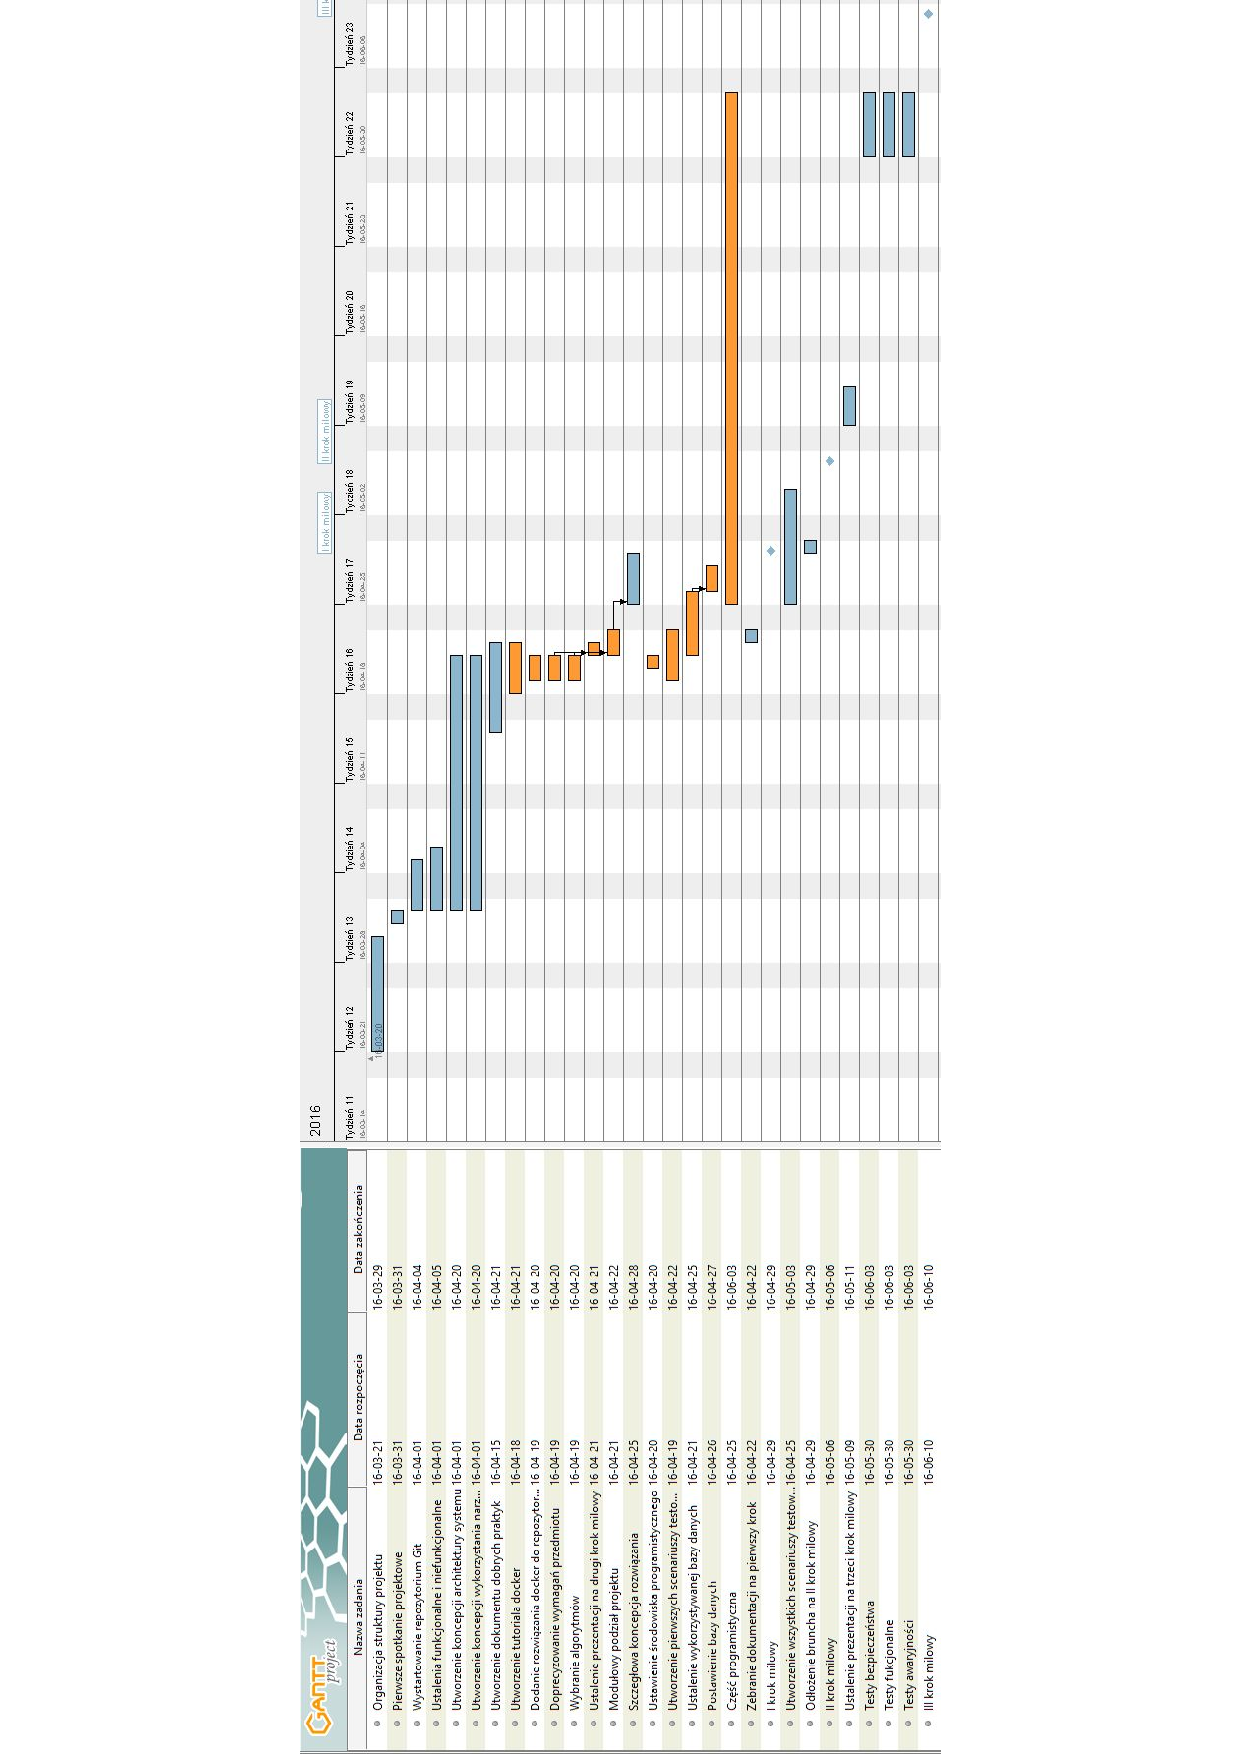
\includepdf[pages={1}]{pdf/gantt.pdf}

\chapter{Wymagania}



\section{Wymagania funkcjonalne}

%\begin{table}[!h]
%\label{tab:fr}
  %\begin{center}
  \begin{longtable}{| p{.20\textwidth} || p{.70\textwidth} |} 
\hline
\textbf{Identyfikator wymagania} & \textbf{Opis wymagania} \\ \hline
FR1 & System umożliwia wyświetlenie listy dostępnych do pobrania wyników badań medycznych \\ \hline
FR2 & System umożliwia pobranie zanonimizowanych wyników badań medycznych
 \\ \hline
FR3 & System umożliwia pobranie statystyk wykonanych badań medycznych
 \\ \hline
  \end{longtable} 
  %\end{center}
%\end{table}

\section{Wymagania niefunkcjonalne}

%\begin{table}[!h]
%\label{tab:nfr}
  %\begin{center}
  \begin{longtable}{| p{.20\textwidth} || p{.70\textwidth} |} 
\hline
\textbf{Identyfikator wymagania} & \textbf{Opis wymagania} \\ \hline
NFR1 & Współbieżne oprogramowanie realizujące część serwerową \\ \hline
NFR2 & Uszkodzenie węzła, nie powoduje zatrzymania pracy systemu
 \\ \hline
NFR3 & Realizacja usługi w trakcie awarii w czasie obsługi
 \\ \hline
NFR4 & Możliwość ponownego wpięcia węzła, z którym utracono łączność
 \\ \hline
NFR5 & Odporność na próbę wpięcia wrogiego, nieuprawnionego węzła
 \\ \hline
NFR6 & Zarządzanie zasobami transparentnie dla oprogramowania klienckiego
 \\ \hline
NFR7 & Zapewnienie poziomu redundancji danych równego 2
 \\ \hline
NFR8 & Maksymalna objętość przechowywanych wszystkich danych równa 1GB
 \\ \hline
NFR9 & Dane o pacjentach oraz badaniach przechowywane w relacyjnej bazie danych PostrgreSQL
 \\ \hline
NFR10 & Wyniki badań medycznych przechowywane w plikach formatu .xml lub .bmp na serwerze danych
 \\ \hline
NFR11 & Uruchamianie i zamykanie części serwerowej jednokrotnym wywołaniem skryptu dowolnym węźle
 \\ \hline
NFR12 & Liczba jednocześnie obsłużonych użytkowników równa 100
 \\ \hline
NFR13 & System uruchamiany w środowisku Linux Ubuntu 14.04 LTS
 \\ \hline
NFR14 & Dwa serwery danych, każdy posiada procesor z minimum czterema wątkami sprzętowymi oraz dyskiem twardym o pojemności min. 20 GB
 \\ \hline
NFR15 & Klaster trzech serwerów (nie wliczając serwerów danych), każdy posiada     procesor z minimum dwoma wątkami sprzętowymi
 \\ \hline
  \end{longtable}  
  %\end{center}
%\end{table}
\chapter{Architektura}

\section{Opis ogólny architektury systemu}

\begin{figure}[!h]
    \begin{center}
    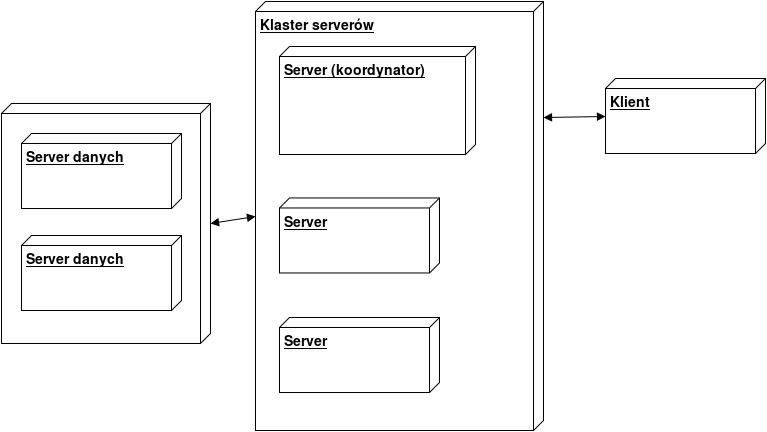
\includegraphics[angle=0,scale=0.55]{img/arch.png}
    \end{center}
    \caption{\em Schemat architektury systemu}
    \label{fig:arch}
\end{figure}


System po stronie serwerowej składa się z dwóch warstw. Wewnętrznej, która przechowuje wrażliwe informacje medyczne i zewnętrznej udostępniającej informację oprogramowaniu klienckiemu. Część wewnętrzną stanowi system rozproszonej bazy danych, a część zewnętrzną klaster serwerów.

\section{Baza danych}

\begin{figure}[!h]
    \begin{center}
    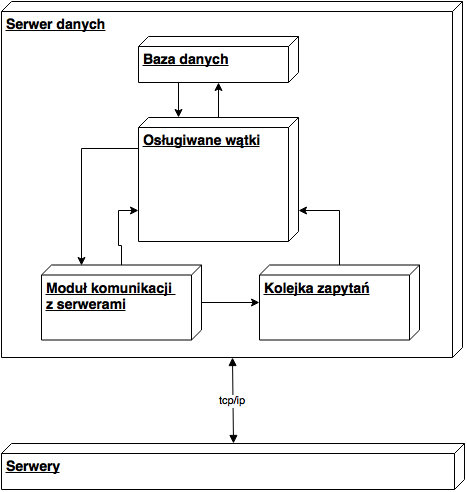
\includegraphics[angle=0,scale=0.75]{img/db.png}
    \end{center}
    \caption{\em Schemat serwera bazy danych}
    \label{fig:db}
\end{figure}

Zastosowany zostanie mechanizm prostej pojedynczej replikacji serwerów danych. Węzły łączą się z wybraną bazą, zapis realizowany jest na dwóch bazach danych jednocześnie.
Przewidziane są dwa serwery danych, co daje redundancję równą 2.

Komunikacja z serwerami odbywa się przez tcp/ip. W komunikacji pośredniczy moduł komunikacyjny, który oczekuje na zapytania. Każde zapytanie jest obsługiwane w oddzielnym wątku. Zapytania są kolejkowane lub odrzucane, gdy zapytań będzie za dużo. Komunikacja jest szyfrowana przy pomocy RSA.


\section{Serwer}

\begin{figure}[!h]
    \begin{center}
    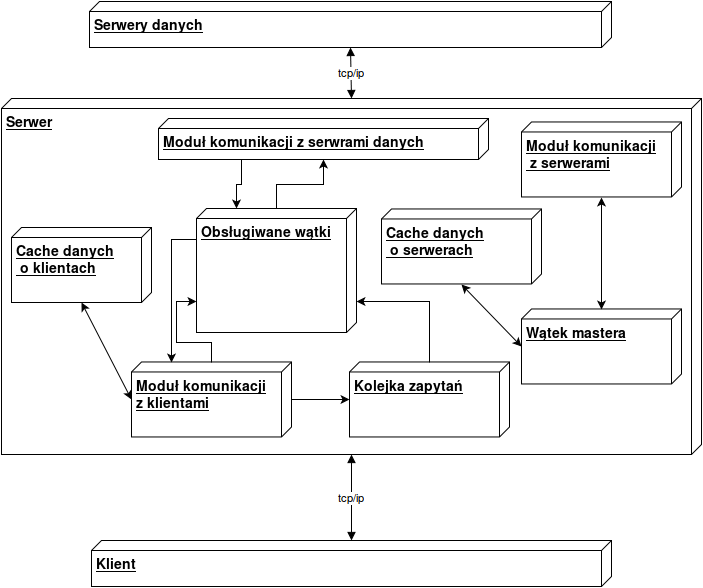
\includegraphics[angle=0,scale=0.6]{img/serv.png}
    \end{center}
    \caption{\em Schemat serwera aplikacyjnego}
    \label{fig:serv}
\end{figure}

Serwer odbiera zapytania od klienta i pobiera dane z bazy. W tym celu nasłuchuje w oczekiwaniu na połączenie od klienta. Komunikacja klient-serwer odbywa się przez tcp/ip. Po odebraniu żądania , tworzony jest nowy wątek, który realizuje zapytanie, komunikuje się z bazą danych oraz formułuje odpowiedź. Serwer może obsłużyć ograniczoną liczbę klientów. Nadmiarowe zapytania może przekazać innym serwerom, a jeżeli wszystkie są zajęte to wstawia do kolejki oczekujących zapytań lub odsyła odpowiedni komunikat, jeżeli w kolejce nie ma miejsc.
Zadaniem serwera jest też autoryzacja łączącego się klienta, sprawdzenie jego uprawnień. Autoryzacja i uwierzytelnienie odbywa się przez podanie loginu i hasła. Gdy serwer dostanie zapytanie od niezalogowanego klienta odsyła prośbę o login i hasło. Po autoryzacji klient jest zapisywany w tablicy aktywnych klientów w pamięci cache, następnie serwer generuje, zapisuje i wysyła token, który będzie służył do uwierzytelniania przy kolejnych żądaniach aż do momentu wylogowania lub gdy użytkownik przez określony czas będzie nieaktywny. Dane o aktywnych klientach nie są przechowywane na wszystkich węzłach, więc jeżeli jeden z nich ulegnie awarii konieczna będzie ponowna autoryzacja i uwierzytelnienie na innym węźle.
Jeden z serwerów jest koordynatorem. Koordynator kontroluje pracę pozostałych serwerów, sprawdza, czy wszystkie są dostępne, autoryzuje nowy węzeł, który chce się połączyć. Tworzy i rozsyła do wszystkich węzłów tablicę aktywności serwerów oraz serwerów danych. Sprawdzanie obecności serwerów odbywa się poprzez cykliczne odpytywanie.
Gdy master ulegnie awarii jego rolę przejmuje inny z serwerów.
Wszystkie serwery znają liczbę i adresy pozostałych. Każdy z serwerów ma przyporządkowany numer. Masterem staje się ten o najniższym numerze. Pierwszy serwer, który zauważy, że nie ma mastera wysyła komunikat do wszystkich węzłów o niższym numerze, jeżeli nikt nie odpowie to serwer staje się nowym koordynatorem i wysyła do wszystkich pozostałych węzłów informujący komunikat. Jeżeli któryś z węzłów o niższym numerze odpowie to on przejmuje kontrolę. Brak koordynatora będzie zauważony, gdy węzeł nie zostanie odpytany w odpowiednim czasie.

\subsection{Autoryzacja węzłów}
Każdy węzeł posiada nazwę oraz numer. Aby dołączyć się do klastra serwerów musi wysłać masterowi numer oraz swoją nazwę zaszyfrowaną kluczem publicznym mastera. W odpowiedzi dostaje potwierdzenie i aktualny stan systemu, aby zaktualizować listę aktywnych serwerów.  Klucze publiczne są zapisywane w plikach konfiguracyjnych serwera i klienta.

\section{Aplikacja kliencka}

\begin{figure}[!h]
    \begin{center}
    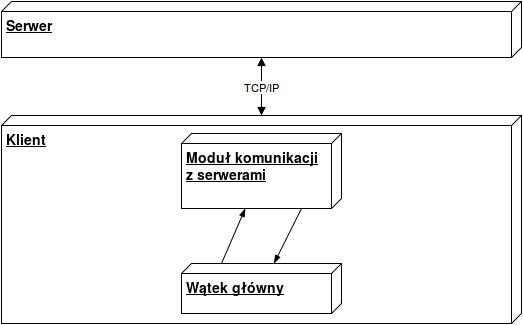
\includegraphics[angle=0,scale=0.8]{img/client.png}
    \end{center}
    \caption{\em Schemat aplikacji klienckiej}
    \label{fig:client}
\end{figure}

Zadaniem aplikacji klienckiej jest nawiązanie połączenia z jednym z serwerów. Adresy serwerów są określone w pliku konfiguracyjnym. Jeżeli połączenie z jednym z węzłów zakończy się niepowodzeniem, następuje próba połączenia się z kolejnymi. Aplikacja umożliwia zalogowanie się i dostęp do funkcji oferowanych przez API serwera. Jeżeli jakieś żądanie się nie powiedzie pomimo dostępności serwera, następuje ponowna próba, wysłania żądania ale do innego serwera.
Klient musi aktualizować listę serwerów poprzez cykliczne odpytywanie.

\section{Plik konfiguracyjny}

W pliku konfiguracyjnym klienta znajdują się adresy, porty i nazwy serwerów oraz ich klucze publiczne.
W pliku konfiguracyjnym serwerów znajdują się adresy, porty i nazwy serwerów, adresy serwerów baz danych, maksymalna liczba jednocześnie obsłużonych wątków, okres odpytywania węzłów przez serwer główny, czas trwania sesji z klientem, klucze publiczne serwerów.
W pliku konfiguracyjnym serwerów danych znajdują się adresy serwerów danych oraz adresy węzłów z ich kluczami publicznymi, liczba maksymalnie obsłużonych wątków.

\chapter{Testy systemu}
\label{ap:2}

\section{Opis testów systemu}

\begin{tabular}{|p{20pt}|p{20pt}|p{20pt}|p{250pt}|p{60pt}|}
	\hline
	\multicolumn{3}{|p{70pt}|}{} & Zaliczony: & TAK/NIE \\ \hline
	1. & & & \multicolumn{2}{|p{310pt}|}{Działanie klienta pobierającego } \\ \hline
	& 1. & & \multicolumn{2}{|p{310pt}|}{Konfiguracja } \\ \hline
	& & 1. & \multicolumn{2}{|p{310pt}|}{Pobranie konfiguracji } \\ \hline
	\multicolumn{3}{|p{70pt}|}{Co sprawdza} & \multicolumn{2}{|p{310pt}|}{Czy lista aktywnych serwerów jest poprawnie pobierana} \\ \hline
	\multicolumn{3}{|p{70pt}|}{Spodziewany efekt} & \multicolumn{2}{|p{310pt}|}{Pobranie listy aktywnych serwerów i zapisanie jej jako nowej konfiguracji} \\ \hline
	\multicolumn{3}{|p{70pt}|}{Jak wykonać} & \multicolumn{2}{|p{310pt}|}{1. Skopiowanie starej wersji pliku konfiguracyjnego 
2. Uruchomienie klienta bez parametrów
3. Sprawdzenie czy plik konfiguracyjny różni się od kopii z 1. punktu (zwłaszcza: czy zawiera więcej niż 1 wpis o serwerach)} \\ \hline
	\multicolumn{3}{|p{70pt}|}{Faktyczny efekt} & \multicolumn{2}{|p{310pt}|}{} \\ \hline
\end{tabular}

\begin{tabular}{|p{20pt}|p{20pt}|p{20pt}|p{250pt}|p{60pt}|}
	\hline
	\multicolumn{3}{|p{70pt}|}{} & Zaliczony: & TAK/NIE \\ \hline
	1. & & & \multicolumn{2}{|p{310pt}|}{Działanie klienta pobierającego } \\ \hline
	& 1. & & \multicolumn{2}{|p{310pt}|}{Konfiguracja } \\ \hline
	& & 2. & \multicolumn{2}{|p{310pt}|}{Łączenie się z zapasowymi serwerami } \\ \hline
	\multicolumn{3}{|p{70pt}|}{Co sprawdza} & \multicolumn{2}{|p{310pt}|}{Czy działa połączenie z innymi serwerami jeśli główny serwer jest wyłączony} \\ \hline
	\multicolumn{3}{|p{70pt}|}{Spodziewany efekt} & \multicolumn{2}{|p{310pt}|}{Połączenie się z pierwszym serwerem który jest dostępny i pobranie wyniku zapytania} \\ \hline
	\multicolumn{3}{|p{70pt}|}{Jak wykonać} & \multicolumn{2}{|p{310pt}|}{1. Uruchomienie klienta bez parametrów (ściągnie się nowa konfiguracja)
2. Wyłączenie serwera, który widnieje w konfiguracji klienta jako pierwszy
3. Uruchomienie klienta do pobrania listy badań)} \\ \hline
	\multicolumn{3}{|p{70pt}|}{Faktyczny efekt} & \multicolumn{2}{|p{310pt}|}{} \\ \hline
\end{tabular}

\begin{tabular}{|p{20pt}|p{20pt}|p{20pt}|p{250pt}|p{60pt}|}
	\hline
	\multicolumn{3}{|p{70pt}|}{FR1} & Zaliczony: & TAK/NIE \\ \hline
	1. & & & \multicolumn{2}{|p{310pt}|}{Działanie klienta pobierającego } \\ \hline
	& 2. & & \multicolumn{2}{|p{310pt}|}{Pobieranie } \\ \hline
	& & 1. & \multicolumn{2}{|p{310pt}|}{Pobranie listy badań } \\ \hline
	\multicolumn{3}{|p{70pt}|}{Co sprawdza} & \multicolumn{2}{|p{310pt}|}{Czy lista dostępnych badań jest pobierana} \\ \hline
	\multicolumn{3}{|p{70pt}|}{Spodziewany efekt} & \multicolumn{2}{|p{310pt}|}{Pobranie listy badań} \\ \hline
	\multicolumn{3}{|p{70pt}|}{Jak wykonać} & \multicolumn{2}{|p{310pt}|}{1. Uruchomienie klienta z parametrem ‘list’} \\ \hline
	\multicolumn{3}{|p{70pt}|}{Faktyczny efekt} & \multicolumn{2}{|p{310pt}|}{} \\ \hline
\end{tabular}

\begin{tabular}{|p{20pt}|p{20pt}|p{20pt}|p{250pt}|p{60pt}|}
	\hline
	\multicolumn{3}{|p{70pt}|}{FR2} & Zaliczony: & TAK/NIE \\ \hline
	1. & & & \multicolumn{2}{|p{310pt}|}{Działanie klienta pobierającego } \\ \hline
	& 2. & & \multicolumn{2}{|p{310pt}|}{Pobieranie } \\ \hline
	& & 2. & \multicolumn{2}{|p{310pt}|}{Pobranie badania o podanym id } \\ \hline
	\multicolumn{3}{|p{70pt}|}{Co sprawdza} & \multicolumn{2}{|p{310pt}|}{Czy pobierane jest wskazane badanie} \\ \hline
	\multicolumn{3}{|p{70pt}|}{Spodziewany efekt} & \multicolumn{2}{|p{310pt}|}{Pobranie pliku przypisanego do badania o podanym id} \\ \hline
	\multicolumn{3}{|p{70pt}|}{Jak wykonać} & \multicolumn{2}{|p{310pt}|}{1. Uruchomienie klienta z parametrem ‘list’ i zapamiętanie jednego z dostępnych numerów id
2. Uruchomienie klienta z parametrem ‘get’
3. Sprawdzenie czy pobrany plik to ten o który chodziło} \\ \hline
	\multicolumn{3}{|p{70pt}|}{Faktyczny efekt} & \multicolumn{2}{|p{310pt}|}{} \\ \hline
\end{tabular}

\begin{tabular}{|p{20pt}|p{20pt}|p{20pt}|p{250pt}|p{60pt}|}
	\hline
	\multicolumn{3}{|p{70pt}|}{FR1} & Zaliczony: & TAK/NIE \\ \hline
	1. & & & \multicolumn{2}{|p{310pt}|}{Działanie klienta pobierającego } \\ \hline
	& 2. & & \multicolumn{2}{|p{310pt}|}{Pobieranie } \\ \hline
	& & 3. & \multicolumn{2}{|p{310pt}|}{Wyszukiwanie badań z filtrowaniem } \\ \hline
	\multicolumn{3}{|p{70pt}|}{Co sprawdza} & \multicolumn{2}{|p{310pt}|}{Czy działa filtrowanie listy dostępnych badań} \\ \hline
	\multicolumn{3}{|p{70pt}|}{Spodziewany efekt} & \multicolumn{2}{|p{310pt}|}{Wyświetlenie listy zawężonej do badań spełniających podane kryteria} \\ \hline
	\multicolumn{3}{|p{70pt}|}{Jak wykonać} & \multicolumn{2}{|p{310pt}|}{1. Uruchomienie klienta z parametrem ‘list’
2. Uruchomienie klienta z parametrem ‘search’ i filtrami: nazwa ‘*’, kraj ‘Polska’, płeć ‘M’, rasa ‘*’, minimalny wiek ‘*’, maksymalny wiek ‘*’
3. Sprawdzenie czy zwrócona lista jest zgodna z zapytaniem z punktu 2
4. Sprawdzenie czy zwrócona lista odpowiada liście z punktu 1 okrojonej do wpisów spełniających podane kryteria} \\ \hline
	\multicolumn{3}{|p{70pt}|}{Faktyczny efekt} & \multicolumn{2}{|p{310pt}|}{} \\ \hline
\end{tabular}

\begin{tabular}{|p{20pt}|p{20pt}|p{20pt}|p{250pt}|p{60pt}|}
	\hline
	\multicolumn{3}{|p{70pt}|}{FR3} & Zaliczony: & TAK/NIE \\ \hline
	1. & & & \multicolumn{2}{|p{310pt}|}{Działanie klienta pobierającego } \\ \hline
	& 2. & & \multicolumn{2}{|p{310pt}|}{Pobieranie } \\ \hline
	& & 4. & \multicolumn{2}{|p{310pt}|}{Pobranie statystyk z filtrowaniem i grupowaniem } \\ \hline
	\multicolumn{3}{|p{70pt}|}{Co sprawdza} & \multicolumn{2}{|p{310pt}|}{Czy pobierane są statystyki spełniające kryteria} \\ \hline
	\multicolumn{3}{|p{70pt}|}{Spodziewany efekt} & \multicolumn{2}{|p{310pt}|}{Pobranie statystyk zgodnych z podanym filtrem i odpowiednio pogrupowanych} \\ \hline
	\multicolumn{3}{|p{70pt}|}{Jak wykonać} & \multicolumn{2}{|p{310pt}|}{1. Uruchomienie klienta z parametrem ‘search’ i filtrami: nazwa ‘*’, kraj ‘Polska’, płeć ‘*’, rasa ‘*’, minimalny wiek ‘*’, maksymalny wiek ‘*’
2. Uruchomienie klienta z parametrem ‘stats’ i filtrami: nazwa ‘*’, kraj ‘Polska’, płeć ‘*’, rasa ‘*’, minimalny wiek ‘*’, maksymalny wiek ‘*’ oraz grupowaniem po płci (‘p’)
3. Sprawdzenie czy statystyki zgadzają się z wynikami z punktu 1} \\ \hline
	\multicolumn{3}{|p{70pt}|}{Faktyczny efekt} & \multicolumn{2}{|p{310pt}|}{} \\ \hline
\end{tabular}

\begin{tabular}{|p{20pt}|p{20pt}|p{20pt}|p{250pt}|p{60pt}|}
	\hline
	\multicolumn{3}{|p{70pt}|}{FR2} & Zaliczony: & TAK/NIE \\ \hline
	1. & & & \multicolumn{2}{|p{310pt}|}{Działanie klienta pobierającego } \\ \hline
	& 2. & & \multicolumn{2}{|p{310pt}|}{Pobieranie } \\ \hline
	& & 5. & \multicolumn{2}{|p{310pt}|}{Działanie anonimizowania badań } \\ \hline
	\multicolumn{3}{|p{70pt}|}{Co sprawdza} & \multicolumn{2}{|p{310pt}|}{Czy pobierane dane są zanonimizowane} \\ \hline
	\multicolumn{3}{|p{70pt}|}{Spodziewany efekt} & \multicolumn{2}{|p{310pt}|}{Pobranie pliku xml z usuniętymi danymi osobowymi} \\ \hline
	\multicolumn{3}{|p{70pt}|}{Jak wykonać} & \multicolumn{2}{|p{310pt}|}{1. Uruchomienie klienta z parametrem ‘list’ i wybranie jednego z dostępnych id
2. Uruchomienie klienta z parametrem ‘get’ i pobranie pliku xml
3. Sprawdzenie czy plik ma poprawnie usunięte dane osobowe} \\ \hline
	\multicolumn{3}{|p{70pt}|}{Faktyczny efekt} & \multicolumn{2}{|p{310pt}|}{} \\ \hline
\end{tabular}

\begin{tabular}{|p{20pt}|p{20pt}|p{20pt}|p{250pt}|p{60pt}|}
	\hline
	\multicolumn{3}{|p{70pt}|}{NFR2} & Zaliczony: & TAK/NIE \\ \hline
	2. & & & \multicolumn{2}{|p{310pt}|}{Działanie serwerów } \\ \hline
	& 1. & & \multicolumn{2}{|p{310pt}|}{Dołączanie, odłączanie serwerów } \\ \hline
	& & 1. & \multicolumn{2}{|p{310pt}|}{Odłączenie jednego serwera warstwy zewnętrznej } \\ \hline
	\multicolumn{3}{|p{70pt}|}{Co sprawdza} & \multicolumn{2}{|p{310pt}|}{Czy usługa działa po odłączeniu jednego z serwerów warstwy zewnętrznej} \\ \hline
	\multicolumn{3}{|p{70pt}|}{Spodziewany efekt} & \multicolumn{2}{|p{310pt}|}{Odłączenie serwera nie wpływa na poprawne działanie usługi} \\ \hline
	\multicolumn{3}{|p{70pt}|}{Jak wykonać} & \multicolumn{2}{|p{310pt}|}{1. Uruchomienie klienta z parametrem ‘list’ i zapamiętanie listy
2. Odłączenie jednego z serwerów warstwy zewnętrznej (np. tego który jest pierwszy w pliku konfiguracyjnym klienta)
3. Uruchomienie klienta z parametrem ‘list’ i porównanie wyniku z punktem 1} \\ \hline
	\multicolumn{3}{|p{70pt}|}{Faktyczny efekt} & \multicolumn{2}{|p{310pt}|}{} \\ \hline
\end{tabular}

\begin{tabular}{|p{20pt}|p{20pt}|p{20pt}|p{250pt}|p{60pt}|}
	\hline
	\multicolumn{3}{|p{70pt}|}{NFR2} & Zaliczony: & TAK/NIE \\ \hline
	2. & & & \multicolumn{2}{|p{310pt}|}{Działanie serwerów } \\ \hline
	& 1. & & \multicolumn{2}{|p{310pt}|}{Dołączanie, odłączanie serwerów } \\ \hline
	& & 2. & \multicolumn{2}{|p{310pt}|}{Odłączenie jednego serwera danych } \\ \hline
	\multicolumn{3}{|p{70pt}|}{Co sprawdza} & \multicolumn{2}{|p{310pt}|}{Czy usługa działa po odłączeniu jednego z serwerów danych} \\ \hline
	\multicolumn{3}{|p{70pt}|}{Spodziewany efekt} & \multicolumn{2}{|p{310pt}|}{Odłączenie serwera nie wpływa na poprawne działanie usługi} \\ \hline
	\multicolumn{3}{|p{70pt}|}{Jak wykonać} & \multicolumn{2}{|p{310pt}|}{1. Uruchomienie klienta z parametrem ‘list’ i zapamiętanie listy
2. Odłączenie jednego z serwerów danych
3. Uruchomienie klienta z parametrem ‘list’ i porównanie wyniku z punktem 1} \\ \hline
	\multicolumn{3}{|p{70pt}|}{Faktyczny efekt} & \multicolumn{2}{|p{310pt}|}{} \\ \hline
\end{tabular}

\begin{tabular}{|p{20pt}|p{20pt}|p{20pt}|p{250pt}|p{60pt}|}
	\hline
	\multicolumn{3}{|p{70pt}|}{NFR4} & Zaliczony: & TAK/NIE \\ \hline
	2. & & & \multicolumn{2}{|p{310pt}|}{Działanie serwerów } \\ \hline
	& 1. & & \multicolumn{2}{|p{310pt}|}{Dołączanie, odłączanie serwerów } \\ \hline
	& & 3. & \multicolumn{2}{|p{310pt}|}{Wymiana serwerów } \\ \hline
	\multicolumn{3}{|p{70pt}|}{Co sprawdza} & \multicolumn{2}{|p{310pt}|}{Czy usługa działa po całkowitej wymianie serwerów jednej z warstw} \\ \hline
	\multicolumn{3}{|p{70pt}|}{Spodziewany efekt} & \multicolumn{2}{|p{310pt}|}{Wymiana serwerów nie wpływa na poprawne działanie usługi} \\ \hline
	\multicolumn{3}{|p{70pt}|}{Jak wykonać} & \multicolumn{2}{|p{310pt}|}{1. Uruchomienie usługi z 2 serwerami warstwy zewnętrznej (spośród 3)
2. Uruchomienie klienta z parametrem ‘list’ i zapamiętanie listy
3. Dołączenie brakującego serwera i odpięcia pozostałych dwóch
4. Uruchomienie klienta z parametrem ‘list’ i porównanie wyniku z punktem 1} \\ \hline
	\multicolumn{3}{|p{70pt}|}{Faktyczny efekt} & \multicolumn{2}{|p{310pt}|}{} \\ \hline
\end{tabular}

\begin{tabular}{|p{20pt}|p{20pt}|p{20pt}|p{250pt}|p{60pt}|}
	\hline
	\multicolumn{3}{|p{70pt}|}{NFR4} & Zaliczony: & TAK/NIE \\ \hline
	2. & & & \multicolumn{2}{|p{310pt}|}{Działanie serwerów } \\ \hline
	& 1. & & \multicolumn{2}{|p{310pt}|}{Dołączanie, odłączanie serwerów } \\ \hline
	& & 4. & \multicolumn{2}{|p{310pt}|}{Pozostawienie po 1 serwerze każdej warstwy } \\ \hline
	\multicolumn{3}{|p{70pt}|}{Co sprawdza} & \multicolumn{2}{|p{310pt}|}{Czy usługa działa po jeśli zostało tylko po jednym serwerze każdej z warstw} \\ \hline
	\multicolumn{3}{|p{70pt}|}{Spodziewany efekt} & \multicolumn{2}{|p{310pt}|}{Odłączenie serwerów nie wpływa na poprawne działanie usługi} \\ \hline
	\multicolumn{3}{|p{70pt}|}{Jak wykonać} & \multicolumn{2}{|p{310pt}|}{1. Uruchomienie klienta i pobranie listy
2. Odłączenie serwerów (zostaje po jednym dla każdej z warstw)
3. Uruchomienie klienta i pobranie listy} \\ \hline
	\multicolumn{3}{|p{70pt}|}{Faktyczny efekt} & \multicolumn{2}{|p{310pt}|}{} \\ \hline
\end{tabular}

\begin{tabular}{|p{20pt}|p{20pt}|p{20pt}|p{250pt}|p{60pt}|}
	\hline
	\multicolumn{3}{|p{70pt}|}{NFR6} & Zaliczony: & TAK/NIE \\ \hline
	2. & & & \multicolumn{2}{|p{310pt}|}{Działanie serwerów } \\ \hline
	& 2. & & \multicolumn{2}{|p{310pt}|}{Spójność danych } \\ \hline
	& & 1. & \multicolumn{2}{|p{310pt}|}{Odłączenie serwera danych } \\ \hline
	\multicolumn{3}{|p{70pt}|}{Co sprawdza} & \multicolumn{2}{|p{310pt}|}{Czy dane są spójne po przełączeniu się na inny serwer danych} \\ \hline
	\multicolumn{3}{|p{70pt}|}{Spodziewany efekt} & \multicolumn{2}{|p{310pt}|}{Dane są spójne} \\ \hline
	\multicolumn{3}{|p{70pt}|}{Jak wykonać} & \multicolumn{2}{|p{310pt}|}{1. Uruchomienie klienta wrzucającego dane i wrzucenie 1 badania z plikiem
2. Uruchomienie klienta z parametrem ‘list’ i zapamiętanie listy (należy upewnić się że na liście jest nowo dodany plik)
3. Odłączenie serwera danych (najlepiej tego, do którego łączył się klient wrzucający)
4. Uruchomienie klienta z parametrem ‘list’ i porównanie wyniku z punktem 2} \\ \hline
	\multicolumn{3}{|p{70pt}|}{Faktyczny efekt} & \multicolumn{2}{|p{310pt}|}{} \\ \hline
\end{tabular}

\begin{tabular}{|p{20pt}|p{20pt}|p{20pt}|p{250pt}|p{60pt}|}
	\hline
	\multicolumn{3}{|p{70pt}|}{NFR3} & Zaliczony: & TAK/NIE \\ \hline
	2. & & & \multicolumn{2}{|p{310pt}|}{Działanie serwerów } \\ \hline
	& 3. & & \multicolumn{2}{|p{310pt}|}{Elekcja } \\ \hline
	& & 1. & \multicolumn{2}{|p{310pt}|}{Odłączenie koordynatora warstwy zewnętrznej } \\ \hline
	\multicolumn{3}{|p{70pt}|}{Co sprawdza} & \multicolumn{2}{|p{310pt}|}{Czy usługa działa po odłączeniu koordynatora warstwy zewnętrznej} \\ \hline
	\multicolumn{3}{|p{70pt}|}{Spodziewany efekt} & \multicolumn{2}{|p{310pt}|}{Usługa działa poprawnie} \\ \hline
	\multicolumn{3}{|p{70pt}|}{Jak wykonać} & \multicolumn{2}{|p{310pt}|}{1. Uruchomienie usługi i sprawdzenie który z serwerów jest koordynatorem
2. Odłączenie koordynatora} \\ \hline
	\multicolumn{3}{|p{70pt}|}{Faktyczny efekt} & \multicolumn{2}{|p{310pt}|}{} \\ \hline
\end{tabular}

\begin{tabular}{|p{20pt}|p{20pt}|p{20pt}|p{250pt}|p{60pt}|}
	\hline
	\multicolumn{3}{|p{70pt}|}{NFR3} & Zaliczony: & TAK/NIE \\ \hline
	2. & & & \multicolumn{2}{|p{310pt}|}{Działanie serwerów } \\ \hline
	& 3. & & \multicolumn{2}{|p{310pt}|}{Elekcja } \\ \hline
	& & 2. & \multicolumn{2}{|p{310pt}|}{Odłączenie koordynatora warstwy danych } \\ \hline
	\multicolumn{3}{|p{70pt}|}{Co sprawdza} & \multicolumn{2}{|p{310pt}|}{Czy usługa działa po odłączeniu koordynatora warstwy danych} \\ \hline
	\multicolumn{3}{|p{70pt}|}{Spodziewany efekt} & \multicolumn{2}{|p{310pt}|}{Usługa działa poprawnie} \\ \hline
	\multicolumn{3}{|p{70pt}|}{Jak wykonać} & \multicolumn{2}{|p{310pt}|}{1. Uruchomienie usługi i sprawdzenie który z serwerów jest koordynatorem
2. Odłączenie koordynatora} \\ \hline
	\multicolumn{3}{|p{70pt}|}{Faktyczny efekt} & \multicolumn{2}{|p{310pt}|}{} \\ \hline
\end{tabular}

\begin{tabular}{|p{20pt}|p{20pt}|p{20pt}|p{250pt}|p{60pt}|}
	\hline
	\multicolumn{3}{|p{70pt}|}{NFR12} & Zaliczony: & TAK/NIE \\ \hline
	3. & & & \multicolumn{2}{|p{310pt}|}{Wymagania niefunkcjonalne } \\ \hline
	& 1. & & \multicolumn{2}{|p{310pt}|}{Obsłużenie 100 użytkowników jednocześnie } \\ \hline
	& & 1. & \multicolumn{2}{|p{310pt}|}{Zapewnienie działania przy normalnej pracy } \\ \hline
	\multicolumn{3}{|p{70pt}|}{Co sprawdza} & \multicolumn{2}{|p{310pt}|}{Czy usługa działa po odłączeniu koordynatora warstwy danych} \\ \hline
	\multicolumn{3}{|p{70pt}|}{Spodziewany efekt} & \multicolumn{2}{|p{310pt}|}{Usługa działa poprawnie} \\ \hline
	\multicolumn{3}{|p{70pt}|}{Jak wykonać} & \multicolumn{2}{|p{310pt}|}{1. Uruchomienie klienta z parametrem ‘list’ i wybranie jednego z id
2. Włączenie 100 razy (najlepiej współbieżnie) klienta z parametrem ‘get’
3. Sprawdzenie czy każdy klient otrzymał spodziewany plik} \\ \hline
	\multicolumn{3}{|p{70pt}|}{Faktyczny efekt} & \multicolumn{2}{|p{310pt}|}{} \\ \hline
\end{tabular}

\begin{tabular}{|p{20pt}|p{20pt}|p{20pt}|p{250pt}|p{60pt}|}
	\hline
	\multicolumn{3}{|p{70pt}|}{NFR12} & Zaliczony: & TAK/NIE \\ \hline
	3. & & & \multicolumn{2}{|p{310pt}|}{Wymagania niefunkcjonalne } \\ \hline
	& 1. & & \multicolumn{2}{|p{310pt}|}{Obsłużenie 100 użytkowników jednocześnie } \\ \hline
	& & 2. & \multicolumn{2}{|p{310pt}|}{Zapewnienie działania w czasie awarii } \\ \hline
	\multicolumn{3}{|p{70pt}|}{Co sprawdza} & \multicolumn{2}{|p{310pt}|}{Czy usługa działa dla 100 jednoczesnych zapytań gdy pracuje po jednym serwerze z każdej warstwy} \\ \hline
	\multicolumn{3}{|p{70pt}|}{Spodziewany efekt} & \multicolumn{2}{|p{310pt}|}{Usługa działa poprawnie} \\ \hline
	\multicolumn{3}{|p{70pt}|}{Jak wykonać} & \multicolumn{2}{|p{310pt}|}{1. Uruchomienie klienta z parametrem ‘list’ i wybranie jednego z id
2. Włączenie klienta z parametrem ‘get’ i zapamiętanie pliku
3. Wyłączenie prawie wszystkich serwerów (zostaje po 1 serwerze każdej warstwy)
4. Włączenie 100 razy (najlepiej współbieżnie) klienta z parametrem ‘get’
5. Sprawdzenie czy każdy klient otrzymał poprawny plik} \\ \hline
	\multicolumn{3}{|p{70pt}|}{Faktyczny efekt} & \multicolumn{2}{|p{310pt}|}{} \\ \hline
\end{tabular}

\begin{tabular}{|p{20pt}|p{20pt}|p{20pt}|p{250pt}|p{60pt}|}
	\hline
	\multicolumn{3}{|p{70pt}|}{NFR11} & Zaliczony: & TAK/NIE \\ \hline
	3. & & & \multicolumn{2}{|p{310pt}|}{Wymagania niefunkcjonalne } \\ \hline
	& 2. & & \multicolumn{2}{|p{310pt}|}{Start i stop usługi } \\ \hline
	& & 1. & \multicolumn{2}{|p{310pt}|}{Start usługi } \\ \hline
	\multicolumn{3}{|p{70pt}|}{Co sprawdza} & \multicolumn{2}{|p{310pt}|}{Czy usługa uruchomi się po wydaniu polecenia na dowolnym z węzłów} \\ \hline
	\multicolumn{3}{|p{70pt}|}{Spodziewany efekt} & \multicolumn{2}{|p{310pt}|}{Usługa uruchamia się na każdym z węzłów} \\ \hline
	\multicolumn{3}{|p{70pt}|}{Jak wykonać} & \multicolumn{2}{|p{310pt}|}{1. Włączenie usługi na jednym z węzłów
2. Sprawdzenie czy usługa jest włączona na każdym z węzłów} \\ \hline
	\multicolumn{3}{|p{70pt}|}{Faktyczny efekt} & \multicolumn{2}{|p{310pt}|}{} \\ \hline
\end{tabular}

\begin{tabular}{|p{20pt}|p{20pt}|p{20pt}|p{250pt}|p{60pt}|}
	\hline
	\multicolumn{3}{|p{70pt}|}{NFR11} & Zaliczony: & TAK/NIE \\ \hline
	3. & & & \multicolumn{2}{|p{310pt}|}{Wymagania niefunkcjonalne } \\ \hline
	& 2. & & \multicolumn{2}{|p{310pt}|}{Start i stop usługi } \\ \hline
	& & 2. & \multicolumn{2}{|p{310pt}|}{Stop usługi } \\ \hline
	\multicolumn{3}{|p{70pt}|}{Co sprawdza} & \multicolumn{2}{|p{310pt}|}{Czy usługa wyłączy się po wydaniu polecenia na dowolnym z węzłów} \\ \hline
	\multicolumn{3}{|p{70pt}|}{Spodziewany efekt} & \multicolumn{2}{|p{310pt}|}{Usługa wyłącza się na każdym z węzłów i zwalnia zajęte porty} \\ \hline
	\multicolumn{3}{|p{70pt}|}{Jak wykonać} & \multicolumn{2}{|p{310pt}|}{1. Włączenie usługi
2. Wydanie polecenia zatrzymania usługi na dowolnym z węzłów (najlepiej na innym niż włączenie usługi)
3. Sprawdzenie czy na każdym węźle usługa jest wyłączona i czy porty są zwolnione
4. Ponowne włączenie usługi i sprawdzenie czy start jest bezproblemowy} \\ \hline
	\multicolumn{3}{|p{70pt}|}{Faktyczny efekt} & \multicolumn{2}{|p{310pt}|}{} \\ \hline
\end{tabular}
\chapter{Docker}

\section{Opis rozwiązania Docker}

Docker jest narzędziem ułatwiającym proces tworzenia, dystrybucji i wdrażania oprogramowania. Pozwala on na umieszczenie aplikacji wraz z jej bezpośrednimi zależnościami w kontenerze i uruchomienie jej na dowolnej maszynie z systemem Linux. Aplikacje działające za pomocą Dockera są odizolowane od infrastruktury, dzięki czemu możliwe jest uruchomienie kilku niezależnych kontenerów z aplikacjami symulujących pracę w środowisku rozproszonym. Jednocześnie narzędzie to zapewnia niewielkie zużycie pamięci dzięki współdzieleniu warstw UFS obrazów (ang. Union File System) pomiędzy kontenerami. Współdzielenie jądra systemu pomiędzy kontenerami, a systemem gospodarza zapewnia natomiast krótkie czasy uruchomienia. Ze względu na te cechy korzystanie z aplikacji uruchomionej za pomocą Dockera jest niemal tak wydajne, jak działającej na systemie gospodarza.

	Podstawowymi komponentami Dockera są:
\begin{itemize}
\item \textit{Docker Engine} -  platforma do tworzenia kontenerów na uruchamiane przez użytkownika aplikacje,
\item \textit{Docker Hub} – oficjalne repozytorium obrazów przechowujące obrazy udostępniane przez użytkowników
\end{itemize}

	Docker działa w architekturze klient – serwer. Do komunikacji klienta z demonem wykorzystywany jest protokół HTTP i odbywa się ona poprzez gniazda (ang. sockets) lub RESTful API. Klient Dockera jest podstawowym interfejsem komunikacyjnym z Dockerem – przyjmuje komendy z określonego zestawu poleceń wpisywane przez użytkownika i przekazuje je do demona. Demon odpowiada za budowanie obrazów, uruchamianie i dystrybucję kontenerów. Klient i demon mogą działać na tym samym systemie lub ich funkcje mogą zosać rozdzielone pomiędzy różne hosty.

Podstawowymi pojęciami Dockera są:
\begin{itemize}
\item \textit{obrazy} – komponent  odpowiadający budowaniu,
\item \textit{rejestry} – komponent odpowiadający dystrybucji,
\item \textit{kontenery} – komponent odpowiadający uruchamianiu.
\end{itemize}

	\textbf{\underline{Obraz}} jest to szablon służący tylko do odczytu, stanowiący podstawę do utworzenia kontenera. Obraz może zawierać np. system operacyjny Ubuntu z serwerem Apache oraz zainstalowaną aplikacją webową, którą chcemy uruchomić. Za pomocą Dockera mamy możliwość budowania nowych obrazów, aktualizowania istniejących, pobierania obrazów stworzonych przez innych i udostępniania własnych. Każdy obraz składa się z warstw tworzących ujednolicony system plików (\textit{ang. UFS}).  Ta technologia powoduje, że obrazy Dockera są lekkie – wprowadzenie zmian w aplikacji nie wiąże się z przebudową całego obrazu, a jedynie z aktualizacją lub dodaniem danej warstwy.
	
	Każdy obraz ma obraz bazowy (np. obraz systemu Ubuntu lub obraz utworzony przez użytkownika), na podstawie którego jest budowany za pomocą zestawu instrukcji. Każda instrukcja powoduje dodanie warstwy do naszego obrazu (taką instrukcją może być np. wywołanie komendy, dodanie pliku lub folderu, instalacja pakietu, utworzenie zmiennej środowiskowej). Polecenia tworzące obraz Dockera przechowywane są w pliku Dockerfile. Podczas budowania obrazu Docker odczytuje kod żródłowy zawarty w pliku Dockerfile, wykonuje zapisane instrukcje i zwraca końcowy obraz.

Przykładowe operacje na obrazie:
\begin{itemize}
\item Pobieranie obrazu:
\begin{lstlisting}[style=incode]
docker pull {nazwa obrazu}
\end{lstlisting}
\item Wyświetlanie lokalnie dostępnych obrazów:
\begin{lstlisting}[style=incode]
docker images
\end{lstlisting}
\item Wyświetlenie warstw składających się na obraz:
\begin{lstlisting}[style=incode]
docker history {id lub nazwa obrazu}
\end{lstlisting}
\item Usunięcie obrazu
\begin{lstlisting}[style=incode]
docker  rmi {id lub nazwa obrazu}
\end{lstlisting}
	
\end{itemize}

	\textbf{\underline{Rejestry}} są miejscem gdzie można udostępniać i skąd można pobierać obrazy. Mogą one być zarówno publiczne, jak i prywatne.  Publiczny rejestr Dockera stanowi Docker Hub zawierający bazę obrazów stworzonych przez użytkowników Dockera. Istnieje również lokalne repozytorium na maszynie użytkownika. Za pomocą klienta Dockera możliwe jest przeszukiwanie opublikowanych obrazów oraz pobieranie ich w celu utworzenia kontenera. 
	
	\textbf{\underline{Kontener}} tworzony jest na podstawie obrazu, który zawiera informacje o tym, co przechowuje kontener, jaki proces ma zostać uruchomiony po jego utworzeniu oraz inne dane konfiguracyjne. Kontener składa się z zestawu ujednoliconych warstw tylko do odczytu, pochodzących z obrazu kontenera oraz z pojedynczej warstwy do odczytu i zapisu umożliwiającej działanie procesów uruchamianych w kontenerze. Na kontenerach można wykonywać podstawowe operacje: uruchomić, zatrzymać, przenieść i usunąć.

Przykładowe operacje na kontenerze
\begin{itemize}
\item Tworzenie i uruchamianie kontenera:
\begin{lstlisting}[style=incode]
docker runl {nazwa lub id obrazu}
\end{lstlisting}
Uruchomienie tego polecenia z parametrem -d powoduje uruchomienie kontenera działającego w tle, natomiast parametr –rm=true powoduje, że kontener zostanie usunięty natychmiast po wykonaniu zadania.
\item Wyświetlanie wszystkich kontenerów:
\begin{lstlisting}[style=incode]
docker ps -a
\end{lstlisting}
\item Zatrzymanie kontenera
\begin{lstlisting}[style=incode]
docker stop {id lub nazwa kontenera}
\end{lstlisting}
\item Usunięcie kontenera
\begin{lstlisting}[style=incode]
docker rm {id lub nazwa kontenera}
\end{lstlisting}
\end{itemize}

	Docker udostępnia również możliwość automatycznego budowania obrazu w synchronizacji z systemem kontroli wersji (GitHub lub Bitbucket). Dzięki umieszczeniu w repozytorium pliku \textit{Dockerfile} oraz powiązaniu konta DockerHub I kontem w wybranym systemie kontroli wersji, po każdorazowej aktualizacji kodu w repozytorium budowany, na jego podstawie budowany jest aktualny obraz Dockera i zapisywany w repozytorium DockerHub.
	
	
	
	
\section{Raport z przykładowych uruchomień}

\subsection{Uruchomienie aplikacji \textit{'Hello World'}}
Aplikacja uruchamiana jest poleceniem
\begin{lstlisting}[style=incode]
$ docker run ubuntu /bin/echo 'Hello world'
\end{lstlisting}
gdzie:
\begin{itemize}
\item \textit{docker run} – uruchamia kontener
\item \textit{ubuntu} – obraz, na podstawie którego tworzony jest kontener (obraz systemu ubuntu)
\item \textit{/bin/echo  'Hello world'} – polecenie, które ma zostać wywołane wewnątrz 	utworzonego kontenera \newline
\end{itemize}
Odpowiedź Dockera na zadaną komendę:
\begin{lstlisting}[style=incode]
Unable to find image 'ubuntu:latest' locally
latest: Pulling from library/ubuntu
759d6771041e: Pull complete
8836b825667b: Pull complete
c2f5e51744e6: Pull complete
a3ed95caeb02: Pull complete
Digest: sha256:b4dbab2d8029edddfe494f42183de20b7e2e871a424ff16ffe7b15a31f102536
Status: Downloaded newer image for ubuntu:latest
Hello world
\end{lstlisting}

Docker przeszukuje dostępne lokalnie obrazy. Jeżeli nie znajduje  danego obrazu lokalnie, wyszukuje i pobiera go z  repozytorium Docker Hub. Następnie uruchamia kontener, wykonuje polecenie wyświetlenia napisu ''Hello world'' I zatrzymuje kontener.


Aplikację można uruchomić również w trybie interaktywnym, stosując flagi -i -t za pomocą polecenia
\begin{lstlisting}[style=incode]
$ docker run -t -i ubuntu /bin/bash
\end{lstlisting}
gdzie flaga - t powoduje uruchomienie terminala w kontenerze, natomiast flaga - i pozwala wczytywać w kontenerze znaki wpisywane na klawiaturze.
Odpowiedź Dockera:
\begin{lstlisting}[style=incode]
root@879d9c1665ca:/# ls
bin   dev  home  lib64  mnt  proc  run   srv  tmp  var boot  etc  lib   media  
opt  root  sbin  sys  usr
root@879d9c1665ca:/# exit
exit
\end{lstlisting}

Innym sposobem uruchomienia aplikacji jest uruchomienie jej w trybie demona dzięki zastosowaniu flagi -d. Poniższe polecenie spowoduje wyświetlenie napisu 'Hello world' co 1 sekundę:
\begin{lstlisting}[style=incode]
$ docker run -d ubuntu /bin/sh -c "while true; do echo hello world; 
sleep 1; done"
\end{lstlisting}
Sprawdzenie, czy kontener został uruchomiony: 
\begin{lstlisting}[style=incode]
$ docker ps
\end{lstlisting}
Odpowiedź Dockera:
\begin{lstlisting}[style=incode]
CONTAINER ID     IMAGE      COMMAND                  CREATED             
STATUS              PORTS               NAMES
c99a2503f886   ubuntu     ''/bin/sh -c 'while tr''   2 minutes ago     
Up 2 minutes                            evil_morse
\end{lstlisting}
Sprawdzenie wyjścia kontenera:
\begin{lstlisting}[style=incode]
$ docker logs evil_morse
\end{lstlisting}
Odpowiedź Dockera:
\begin{lstlisting}[style=incode]
hello world
hello world
hello world ....
\end{lstlisting}
Zatrzymanie kontenera:
\begin{lstlisting}[style=incode]
$ docker stop evil_morse
\end{lstlisting}


\subsection{Uruchomienie aplikacji webowej}

Aplikacja uruchamiana jest poleceniem:
\begin{lstlisting}[style=incode]
$ docker run -d -P training/webapp python app.py
\end{lstlisting}
gdzie
\begin{itemize}
\item \textit{docker run} – uruchamia kontener
\item \textit{-d} - flaga powodująca działanie w tle kontenera
\item \textit{-P} – flaga nakazująca Dockerowi odwzorowanie portów kontenera na porty na maszynie gospodarza
\item \textit{training/webapp} –  obraz, na podstawie którego tworzony jest kontener
\item \textit{python app.py} – polecenie, które ma zostać wywołane wewnątrz utworzonego kontenera (uruchomienie aplikacji webowej)
\end{itemize}
Odpowiedź Dockera:
\begin{lstlisting}[style=incode]
Unable to find image 'training/webapp:latest' locally
latest: Pulling from training/webapp
e190868d63f8: Pull complete 
909cd34c6fd7: Pull complete 
0b9bfabab7c1: Pull complete 
a3ed95caeb02: Pull complete 
10bbbc0fc0ff: Pull complete 
fca59b508e9f: Pull complete 
e7ae2541b15b: Pull complete 
9dd97ef58ce9: Pull complete 
a4c1b0cb7af7: Pull complete 
Digest: sha256:06e9c1983bd6d5db5fba376ccd63bfa529e8d02f23d5079b8f74a616308fb11d
Status: Downloaded newer image for training/webapp:latest
426c053faa028c411e8ca32f21ec9907da7b442dd83a321f4e47697a8e7cfb7f
\end{lstlisting}
Obraz nie został znaleziony w lokalnym rejestrze, dlatego pobrano go z rejestru Docker Hub. Za pomocą polecenia \textit{docker ps -l} można sprawdzić szczegółowe informacje dotyczące ostatnio uruchomionego kontnera.
\begin{lstlisting}[style=incode]
 $ docker ps -l
CONTAINER ID   IMAGE             COMMAND             CREATED             
STATUS              PORTS                     NAMES
426c053faa02  training/webapp   "python app.py"     13 minutes ago      
Up 12 minutes       0.0.0.0:32768->5000/tcp   berserk_euler
\end{lstlisting}
Kolumna \textit{ports} mówi nam o tym, że port 5000 w kontenerze jest odwzorowany na port 32768 na maszynie lokalnej. Działanie aplikacji możemy sprawdzić wyszukując w przeglądarce port  32768.
\begin{figure}[!h]
    \begin{center}
    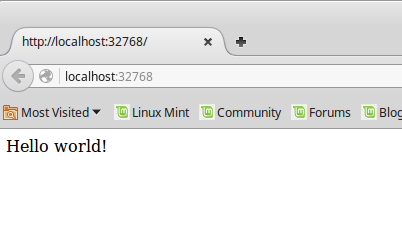
\includegraphics[angle=0,scale=0.75]{img/docker.png}
    \end{center}
    \caption{\em Działająca aplikacja webowa}
    \label{fig:webapp}
\end{figure}

\subsection{Tworzenie własnego obrazu}

Własny obraz można utworzyć na dwa sposoby:
\begin{itemize}
\item Poprzez aktualizację kontenera stworzonego na podstawie obrazu oraz zapisanie wprowadzonych zmian do obrazu
\item Za pomocą pliku \textit{Dockerfile}
\end{itemize}

 W pierwszym przypadku mamy utworzony kontener na podstawie obrazu i wprowadziliśmy do niego nowe dane, np. zainstalowaliśmy program. Nowy obraz tworzymy za pomocą polecenia:
\begin{lstlisting}[style=incode]
$ docker commit -m "Added program" -a "Author" bd625e9176a7 author/ubuntu:v2
\end{lstlisting}
gdzie
\begin{itemize}

\item \textit{docker commit} – zapisuje stn kontenera w postaci obrazu
\item \textit{-m} – flaga pozwalająca zapisać co zostało zmienione w obrazie
\item \textit{-a} – flaga informująca o autorze wprowadzonych zmian
\item \textit{bd625e9176a7} –  numer ID kontenera, na bazie którego tworzony jest nowy obraz
\item \textit{author/ubuntu:v2} – nazwa repozytorium oraz znacznik wersji utworzonego obrazu
\end{itemize}
Po wywołaniu tego polecenia moemy sprawdzić listę obrazów w lokalnym repozytorium:
\begin{lstlisting}[style=incode]
$ docker images
REPOSITORY          	TAG                 IMAGE ID            	     CREATED             	
SIZE
author/ubuntu       	   v2                  adbc62b82a11        19 seconds ago      	
725.1 MB
ubuntu         		  latest              b72889fa879c        11 days ago             	
188 MB
training/webapp   	  latest              6fae60ef3446        11 months ago     	  
348.8 MB 
\end{lstlisting}


Tworzenie obrazu z pliku \textit{Dockerfile} przebiega następująco. Najpierw tworzymy katalog na nasz plik, a w nim plik \textit{Dockerfile}:
\begin{lstlisting}[style=incode]
$ mkdir dockerbuild
$ cd dockerbuild/
$ touch Dockerfile
\end{lstlisting}
Zawartość pliku może wyglądać następująco:
\begin{lstlisting}[style=incode]
FROM ubuntu:14.04
MAINTAINER Author <author@example.com>
RUN apt-get update 
RUN apt-get install build-essential 
RUN apt-get install qt5-default
\end{lstlisting}
Plik \textit{Dockerfile} składa się z instrukcji, których nzwy pisane są wielkimi literami poprzedzających polecenia: \textit{INSTRUKCJA polecenie}. Wyjaśnienie instrukcji wykorzystanych w powyższym pliku:
\begin{itemize}

\item \textit{FROM ubuntu:14.04} – ta komenda mówi o tym, że obraz bazuje na obrazie systemu ubuntu wersji 14.04
\item \textit{MAINTAINER Author <author@example.com>} - wskazanie autora obrazu
\item \textit{RUN ...} - instrukcja RUN nakazuje wykonać w kontenerze dane polecenia
\end{itemize}
Następnie budujemy obraz na podstawie pliku \textit{Dockerfile} (przy wywołaniu tej komendy musimy znajdować się w katalogu, w którym jest nasz plik \textit{Dockerfile}):
\begin{lstlisting}[style=incode]
$ docker build -t author/ubuntu:v2 .
\end{lstlisting}


\subsection{Korzystanie z Docker Hub}

Utworzony obraz może zostac udostępniony w repozytorium Docker Hub, a następnie pobrany przez członków naszego zespołu. W tym celu należy się zalogować na swoje konto Docker Hub za pomoc klienta dockera:
\begin{lstlisting}[style=incode]
$ docker login
\end{lstlisting}
Po podaniu danych logowania możemy udostępnić obraz:
\begin{lstlisting}[style=incode]
$ docker push author/ubuntu:v2
\end{lstlisting}
Następnie może on zostać pobrany przez innch użytkowników:
\begin{lstlisting}[style=incode]
$ docker pull author/ubuntu:v2
\end{lstlisting}

\nocite{*}


\begin{appendices}
\makeatletter
\renewcommand*\FormatBlockHeading[1]{%
  \leftskip\@titleindent
  #1{\noindent
  \ifHeadingNumbered
    \@chapapp\ \mw@seccntformat\HeadingNumber
  \fi
  \ignorespaces\HeadingText\@@par}
  }
\makeatother
\chapter{Wprowadzenie i instrukcja użytkowania systemu kontroli wersji Git}
\label{ap:1}

\section{Wprowadzenie}

Do wspomagania równoległego, rozgałęzionego procesu rozwoju projektu przez wielu programistów, zdecydowano się wykorzystać rozproszony system kontroli wersji Git. 

	Git jest obecnie najbardziej popularną implementacją rozproszonego systemu kontroli wersji. W przeciwieństwie do innych systemów kontroli wersji, Git nie zapamiętuje zmian między kolejnymi rewizjami, lecz kompletne obrazy. Każdy z użytkowników posiada lokalną kopię repozytorium na swoim własnym komputerze po uprzednim sklonowaniu repozytorium zewnętrznego (zdalnego).  Pozwala to na pracę w trybie off-line i wprowadzanie zmian w wersji lokalnej projektu i efektywną pracę nad dużymi projektami.
	
\begin{figure}[!h]
    \begin{center}
    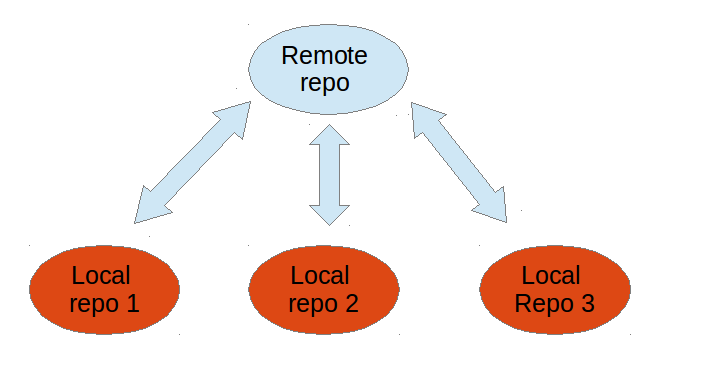
\includegraphics[angle=0,scale=0.5]{img/repo.png}
    \end{center}
    \caption{\em Schemat połączeń między repozytoriami Git}
    \label{fig:repo}
\end{figure}

Następnie zmiany mogą być wymieniane między lokalnymi repozytoriami. Służy do tego repozytorium zewnętrzne (remote repository) działające na serwerze. Serwisem przechowującym rozwijany projekt jest GitHub (\url{https://github.com/}), który udostępnia darmowy hosting open source. 


Repozytorium projektu jest dostępne pod adresem: \url{https://github.com/Gonz8/RSO-16L}

\section{Przygotowanie do pracy i pierwsze pobranie zawartości repozytorium}
	Na samym początku wymagane jest posiadanie klienta Git zainstalowanego w swoim systemie. Wszelkie istotne informacje dotyczące korzystania z Git możemy uzyskać wpisując w terminalu:
\begin{lstlisting}[style=incode]
$ git help
\end{lstlisting}
Następnie musimy określić własną nazwę oraz adres e-mail w systemie Git:
\begin{lstlisting}[style=incode]
$ git config --global user.name ''Your Name''
$ git config --global user.email ''address@example.com''
\end{lstlisting}
Aby zaimportować repozytorium ze wspomnianego serwera należy wykonać polecenie:
\begin{lstlisting}[style=incode]
$ git clone https://github.com/Gonz8/RSO-16L
\end{lstlisting}
Wszystkie pliki zostaną sklonowane do nowo utworzonego katalogu, z poziomu którego należy utworzyć lokalne repozytorium:
\begin{lstlisting}[style=incode]
$ git init
\end{lstlisting}
Utworzone w ten sposób repozytorium jest już powiązane ze zdalną wersją (origin). Możemy to sprawdzić przy użyciu polecenia:
\begin{lstlisting}[style=incode]
$ git remote -v
\end{lstlisting}

\section{Użytkowanie}

Po zaimportowaniu projektu oraz utworzeniu lokalnej kopii repozytorium można rozpocząć pracę z danymi. Aby sprawdzić status dokonanych zmian należy użyć w katalogu z kopią roboczą następującego polecenia:
\begin{lstlisting}[style=incode]
$ git status
\end{lstlisting}
Dodanie nowego pliku, kilku plików lub katalogu do kopii roboczej wykonywane jest przy użyciu komendy:
\begin{lstlisting}[style=incode]
$ git add <filename>
$ git add *
\end{lstlisting}
Aby zatwierdzić wszelkie dokonane zmiany w lokalnym repozytorium należy użyć polecenia:
\begin{lstlisting}[style=incode]
$ git commit -a
\end{lstlisting}
a następnie podać treść/opis poczynionych zmian.
W celu przechwycenia najnowszych zmian z serwera wykonujemy polecenie:
\begin{lstlisting}[style=incode]
$ git fetch origin
\end{lstlisting}
natomiast, aby przechwycić zmiany z serwera i dodatkowo dołączyć je do własnego katalogu roboczego wykonujemy polecenie:
\begin{lstlisting}[style=incode]
$ git pull
\end{lstlisting}

Wysłanie zmian poczynionych w wersji lokalnej do zdalnego repozytorium realizowane jest dzięki komendzie:
\begin{lstlisting}[style=incode]
$ git push origin master
$ git push origin <branchname>
\end{lstlisting}
Git pozwala również na tworzenie, usuwanie i przełączanie się między gałęziami projektu, do wykonania tych operacji służą następujące polecenia:
\begin{lstlisting}[style=incode]
$ git checkout -b <branchname>
$ git branch -d <branchname>
$ git checkout <branchname>
\end{lstlisting}
Wyświetlenie listy wszystkich gałęzi dostępnych w repozytorium możliwe jest poprzez komendę:
\begin{lstlisting}[style=incode]
$ git branch
\end{lstlisting}
Natomiast w celu dołączenia innej gałęzi do obecnie aktywnej należy wykonać polecenie:
\begin{lstlisting}[style=incode]
$ git merge <branchname>
\end{lstlisting}

Ostatnim również istotnym poleceniem jest wyświetlenie historii logów/commit'ów:
\begin{lstlisting}[style=incode]
$ git log
\end{lstlisting}

Dodatkowo po zainstalowaniu pakietu \textit{\textbf{gitk}} można wyświetlać graficzną prezentację historii zmian projektu.

\section{Dodatkowe narzędzia}
	Mimo faktu, że Git jest rozproszonym systemem kontroli wersji, zdecydowano się na wykonywanie dodatkowej i okresowej kopii zapasowej projektu (tzw. backup). Kopia bezpieczeństwa jest jednym z elementów utrzymania repozytorium i zabezpiecza przed utratą danych (np. awarii może ulec komputer głównego programisty, przez co istnieje ryzyko utraty lokalnej kopii repozytorium). Rozwiązaniem tego zagadnienia będzie okresowe wywoływanie napisanego skryptu, który aktualizuje zawartość sklonowanego repozytorium znajdującego się również w folderze powiązanym z naszym kontem Dropbox. Pozwala to w prosty sposób przechowywać kopię zawartości repozytorium na innym serwerze zewnętrznym (poza GitHub) i zabezpieczyć przed utratą danych.

Serwis GitHub świadczy szereg dodatkowych usług wspomagających rozwój projektu programistycznego. Zdecydowano się wykorzystać usługę Wiki, gdzie w łatwy sposób można wprowadzać i modyfikować istotne treści w kontekście projektu. Jest to miejsce, gdzie można w szybki i wygodny sposób odnaleźć uporządkowane informacje. Jednym z odnośników w tej usłudze jest zakładka ''Dobre praktyki kodowania'', gdzie znajdują się wszystkie wspólnie ustalone przez programistów zasady pisania kodu pozwalające utrzymać przejrzystość i spójność kodu.

	Ponadto zdecydowano się uruchomić usługę śledzenia zgłoszeń (tzw. \textit{issue tracking}) na potrzeby wspierania testowania oprogramowania oraz zgłaszania napotkanych błędów i tworzenia dla nich poprawek.

\section{Przydatne informacje}
Instrukcja została opracowana na postawie materiałów znalezionych w sieci. Więcej informacji dotyczących użytkowania systemu kontroli wersji Git można znaleźć na stronach:
\begin{itemize}
\item \url{https://git-scm.com/docs/gittutorial}
\item \url{http://www.vogella.com/tutorials/Git/article.html\#git}
\end{itemize}
\chapter{Spotkania zespołu}
\label{ap:2}

Poniżej znajduje się lista spotkań zespołu (z datami i ustaleniami):

\section{Spotkanie zespołu nr 1}

\textbf{Data spotkania:}  31 marca 2016

\textbf{Ustalenia:}

\begin{itemize}
\item Przedstawienie oczekiwań wobec ról w projekcie
\item Interpretacja i doprecyzowanie tematu projektu
\item Wybór danych medycznych jako danych przetwarzanych w ramach projektu
\item Przydział zadań na najbliższy czas:
	\begin{itemize}
	\item Dominik Giżyński - założenie repozytorium, instrukcja korzystania oraz dokument dobrych praktyk obowiązujących w projekcie
	\item Piotr Kuciński - doprecyzowanie wymagań przedmiotu, przegląd algorytmów do wykorzystania w projekcie
	\item Włodzimierz Szewczyk - doprecyzowanie wymagań przedmiotu, przegląd algorytmów do wykorzystania w projekcie
	\item Michał Herman - szkielet dokumentacji, wybór bazy danych używanej w projekcie
	\item Magda Malenda - architektura systemu, podział systemu na moduły, specyfikacja wymagań, wybór bazy danych używanej w projekcie
	\item Joanna Ohradka - koncepcja wykorzystania narzędzia Docker
	\item Tomasz Rydzewski - harmonogram projektu, specyfikacja wymagań
	\end{itemize}
\end{itemize}



\section{Spotkanie zespołu nr 2}

\textbf{Data spotkania:} 19 kwietnia 2016

\textbf{Ustalenia:}

\begin{itemize}
\item Porzucenie pomysłu klastrowej bazy danych
\item Definiowanie zadań na drugi etap
\item Spisanie koncepcji architektury, wymagań i zastosowania Dockera (do 23 kwietnia)
\item Zebranie i ujednolicenie dokumentacji (do 27 kwietnia)
\end{itemize}


\section{Spotkanie zespołu nr 3}

\textbf{Data spotkania:} 10 maja 2016

\textbf{Ustalenia:}

\begin{itemize}
\item Omówienie poprawek do etapu pierwszego
\item Cotygodniowe spotkania (termin wybrany później ankietą)
\item W przypadku potrzeby częstszych spotkań w mniejszym gronie - telekonferencje
\item Ustalenie rodzaju przetwarzania danych : statystyka i anonimizacja
\item Przeniesienie komunikacji w ramach zadań na GitHub
\item Przydział zadań na drugi etap:
	\begin{itemize}
	\item Dominik Giżyński - prototyp aplikacji
	\item Piotr Kuciński - plan testów
	\item Włodzimierz Szewczyk - uruchamianie / zatrzymywanie aplikacji, scenariusz końcowej demonstracji projektu
	\item Michał Herman - zebranie poprawionych dokumentacji pierwszego etapu, zredagowanie ustaleń ze spotkań zespołu, wyszukanie aktów prawnych dotyczących ochrony danych osobowych, wygenerowanie przykładowych danych do bazy
	\item Magda Malenda - szczegółowy opis rozwiązania, protokół komunikacyjny
	\item Joanna Ohradka - protokół spójności, szkolenia Docker
	\end{itemize} 
\end{itemize}

\section{Spotkanie zespołu nr 4}

\textbf{Data spotkania:} 17 maja 2016

\textbf{Ustalenia:}

\begin{itemize}
\item Omówienie postępu prac
\item Harmonogram na następne dwa tygodnie (do końca drugiego etapu):
	\begin{itemize}
	\item Interfejs protokołu komunikacyjnego (do 20 maja) - osoby odpowiedzialne : Piotr Kuciński i Magda Malenda
	\item Poprawiona i uzupełniona dokumentacja, raport z postępu prac (do 26 maja) - Michał Herman
	\item Połączenie poszczególnych modułów (24 maja) - Dominik Giżyński i Włodzimierz Szewczyk
	\end{itemize}
\item Potrzeba środowiska wirtualnego (przygotowanie maszyny wirtualnej - Piotr Kuciński)
\end{itemize}


\section{Spotkanie zespołu nr 5}

\textbf{Data spotkania:} 24 maja 2016

\textbf{Ustalenia:}

\begin{itemize}
\item Dwie wersje klienta (jedna pobierająca - komunikuje się z serwerami warstwy zewnętrznej, druga dodająca/usuwająca dane z bazy - komunikuje się bezpośrednio z serwerami warstwy wewnętrznej).
\item Przydział kolejnych zadań:
	\begin{itemize}
	\item Piotr Kuciński - klient
	\item Joanna Ohradka - protokół spójności
	\item Magda Malenda - węzeł warstwy wewnętrznej (bez statystyki danych)
	\item Włodzimierz Szewczyk - prezentacja końcowa
	\item Dominik Giżyński - węzeł warstwy zewnętrznej
	\item Michał Herman - zasilenie bazy danych przykładowymi danymi, statystyka
	\end{itemize}
\end{itemize}
\chapter{Narzędzia}
\label{ap:1}

Poniżej znajduje się lista narzędzi i technologii użytych do realizacji projektu.

\begin{itemize}

\item C++
\item Qt
\item PostgreSQL

\end{itemize}
\chapter{Role projektowe}
\label{ap:4}


\begin{longtable}{| p{.50\textwidth} | p{.50\textwidth} |}
\hline
Imię i Nazwisko & Tomasz Rydzewski \\ \hline
Stanowisko & Kierownik \\ \hline
Prace koncepcyjne & \begin{itemize} 
\item przydział ról
\item organizacja spotkań projektowych 
\item organizacja harmonogramu projektu
\item pomoc w opracowaniu wstępnej architektury \end{itemize} \\ \hline
Prace developerskie & \\ \hline
\end{longtable}

\begin{longtable}{| p{.50\textwidth} | p{.50\textwidth} |}
\hline
Imię i Nazwisko & Joanna Ohradka \\ \hline
Stanowisko & Specjalista Dockera \\ \hline
Prace koncepcyjne & \begin{itemize} 
\item opracowanie wykorzystania rozwiązania docker 
\item stworzenie materiałów szkoleniowych z wykorzystywania 
\item weryfikacja poprawności dokumentacji \end{itemize} \\ \hline
Prace developerskie & \begin{itemize}
\item prace nad protokołem spójności
\item prace nad serwerem warstwy wewnętrznej
\item prace nad klientem do wprowadzania danych
\item debugowanie węzłów oraz klienta
\end{itemize} \\ \hline
\end{longtable}

\begin{longtable}{| p{.50\textwidth} | p{.50\textwidth} |}
\hline
Imię i Nazwisko & Michał Herman \\ \hline
Stanowisko & Dokumentalista/Specjalista od bazy danych \\ \hline
Prace koncepcyjne & \begin{itemize} 
\item spajanie dokumentacji projektowej 
\item weryfikacja poprawności dokumentacji 
\item sporządzanie notatek ze spotkań projektowych \end{itemize} \\ \hline
Prace developerskie & \begin{itemize}
\item prace nad bazą danych
\item integracja serwera warstwy wewnętrznej z bazą danych
\item prace nad wyciąganiem statystyk z danych
\item prace nad anonimizacją danych
\item wypełnienie bazy danych przykładowymi danymi
\item debugowanie węzłów
\end{itemize} \\ \hline
\end{longtable}

\begin{longtable}{| p{.50\textwidth} | p{.50\textwidth} |}
\hline
Imię i Nazwisko & Włodzimierz Szewczyk \\ \hline
Stanowisko & Handlowiec \\ \hline
Prace koncepcyjne & \begin{itemize} 
\item zdobycie podstawowych informacji o przedmiocie projektu 
\item pomoc w opracowaniu przypadków użycia na potrzeby testów
\item przygotowanie prezentacji końcowej projektu \end{itemize} \\ \hline
Prace developerskie & \begin{itemize}
\item prace nad rozruchem aplikacji (połączenie ssh wszystkich hostów)
\item pomoc w implementacji serwera
\item debugowanie węzłów oraz klienta
\end{itemize} \\ \hline
\end{longtable}

\begin{longtable}{| p{.50\textwidth} | p{.50\textwidth} |}
\hline
Imię i Nazwisko & Piotr Kuciński \\ \hline
Stanowisko & Tester \\ \hline
Prace koncepcyjne & \begin{itemize} 
\item audyty koncepcji projektu 
\item prace nad protokołem komunikacyjnym
\item opracowanie planu testów
\item pomoc w opracowaniu planu prezentacji \end{itemize} \\ \hline
Prace developerskie & \begin{itemize}
\item prace nad biblioteką komunikacyjną
\item prace nad klientem do pobierania danych oraz klientem do wstawiania danych
\item debugowanie węzłów oraz klienta
\end{itemize} \\ \hline
\end{longtable}

\begin{longtable}{| p{.50\textwidth} | p{.50\textwidth} |}
\hline
Imię i Nazwisko & Dominik Giżyński \\ \hline
Stanowisko & Repomaster \\ \hline
Prace koncepcyjne & \begin{itemize} 
\item pracę nad algorytmem elekcji
\item utrzymywanie repozytorium
\item stworzenie dokumentacji systemu kontroli wersji git \end{itemize} \\ \hline
Prace developerskie & \begin{itemize}
\item prace nad serwerem warstwy wewnętrznej
\item implementacja algorytmu elekcji dla obu warstw części serwerowej
\item implementacja serwera warstwy zewnętrznej
\item debugowanie węzłów
\end{itemize} \\ \hline
\end{longtable}

\begin{longtable}{| p{.50\textwidth} | p{.50\textwidth} |}
\hline
Imię i Nazwisko & Magdalena Malenda \\ \hline
Stanowisko & Architekt \\ \hline
Prace koncepcyjne & \begin{itemize} 
\item opracowanie koncepcji architektury
\item opracowanie protokołu komunikacyjnego \end{itemize} \\ \hline
Prace developerskie & \begin{itemize}
\item implementacja serwera warstwy wewnętrznej
\item implementacja biblioteki komunikacyjnej
\item debugowanie węzłów
\end{itemize} \\ \hline
\end{longtable}


\end{appendices}

\end{document}

% ex: set tabstop=4 shiftwidth=4 softtabstop=4 noexpandtab fileformat=unix filetype=tex spelllang=pl,en spell:

